\section{Closed Loop Response}\label{closedLoop}
A first approximation of the system's behavior in closed loop can be done through a proportional controller.

Such a system is tested with a gain of 10 as a controller. \Figref{closedLoopResponse} shows the response of the simulation and the one from the real setup under a similar fall test as in \appref{fallResponseAppendix}. 

\begin{figure}[H] 
	\centering 
	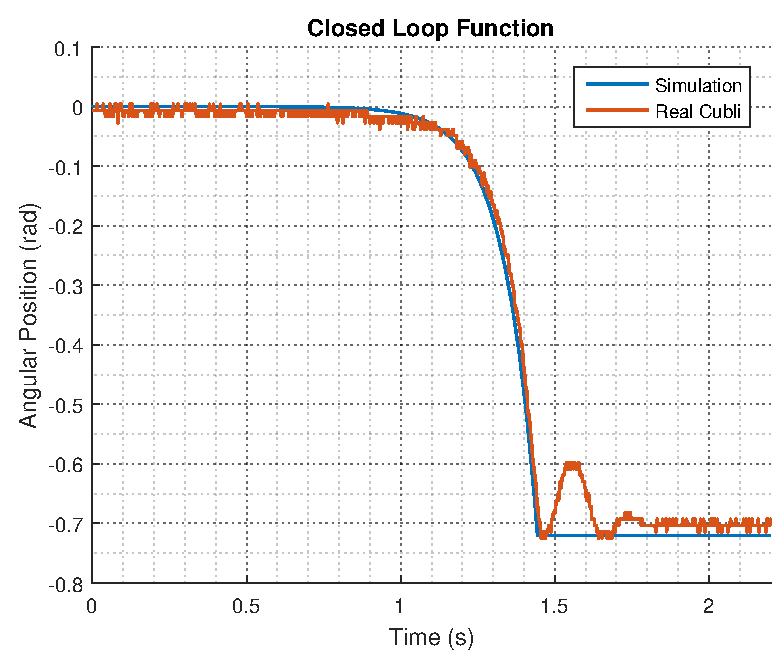
\includegraphics[scale=0.6]{figures/closedLoopResponse}	
	\caption{Behavior of the closed loop function with a proportional controller, both in simulation and reality}
	\label{closedLoopResponse}
\end{figure}
%
It is clear that, upon application of a \SI{0}{rad} reference and a minimal initial offset, the closed loop function with only a gain of 10 has an unstable response.
